\section{Trigonometric Functions} \label{S.0.5.TrigFunctions}


\vspace*{-14 pt}
\framebox{\hspace*{3 pt}
\parbox{6.25 in}{\begin{goals}
\item  How can we model systems that vary in a smooth, wavelike cycle, rising and falling again and again?  
\item How can we model the shape of waves in water, sound waves, radio waves, the motion of the tides in and out over the course of a day, the shaking of an earthquake, or the varying time of sunrise over the course of a year?
\end{goals}} \hspace*{3 pt}}


% \begin{web}
% \item
%     \href{https://www.khanacademy.org/math/trigonometry/unit-circle-trig-func/radians_tutorial/v/introduction-to-radians}{Khan
%     Playlist: Radian measure and arc length}
% \item
%     \href{https://www.khanacademy.org/math/trigonometry/unit-circle-trig-func/Trig-unit-circle}{Khan
%     Playlist: Trig on the unit circle}
% \item
%     \href{https://www.khanacademy.org/math/trigonometry/unit-circle-trig-func/trig-functions-special-angles}{Khan
%     Playlist: Trig functions of special angles}
% \item
%     \href{https://www.khanacademy.org/math/trigonometry/unit-circle-trig-func/inverse_trig_functions}{Khan
%     Playlist: Inverse trig functions}
% \item
%     \href{https://www.khanacademy.org/math/trigonometry/trig-function-graphs/trig_graphs_tutorial/v/midline-amplitude-period}{Khan
%     Playlist: Graphs of trig functions}
% \item
%     \href{https://www.khanacademy.org/math/trigonometry/trig-function-graphs/modeling-periodic-functions}{Khan
%     Playlist: Modeling with periodic functions}
% \end{web}

\nin \hrulefill


\subsection*{Introduction}

You probably first learned about sines, cosines, and tangents when you were studying triangles.  However, these functions are amazingly useful in an enormous variety of contexts.  These functions are so handy that scientists and mathematicians always keep them in mind as part of our standard toolbox.  We use sines and cosines whenever we see anything that varies in a smooth wave cycle, going up and down by the same amount, again and again on a regular basis.

% Your preview activity goes here

\begin{pa} \label{PA:0.5}
A tall water tower is swaying back and forth in the wind.  Using an ultrasonic ranging
device, we measure the distance from our device to the tower (in centimeters) every two
seconds with these measurements recorded below.  

\medskip

\begin{tabular}{| c | c | c | c | c | c | c | c | c | c | c | c |}
\hline
Time (sec) & 0 & 2 & 4 & 6 & 8 & 10 & 12 & 14 & 16 & 18 & 20 \\
\hline
Distance (cm) & 30.9 & 23.1 & 14.7 & 12.3 & 17.7 & 26.7 & 32.3 & 30.1 & 21.8 & 13.9 & 12.6 \\
\hline
\end{tabular}

% \begin{enumerate}
\ba
\item Use the coordinate plane below to create a graph of these data points.
    \begin{center}
        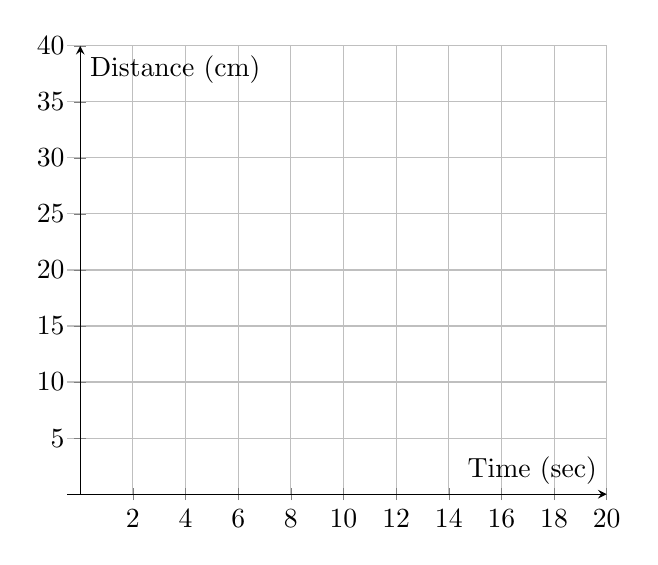
\begin{tikzpicture}
            \begin{axis}[axis lines=center, xmin=-0.5, xmax=20, ymin=0, ymax=40,
                xtick={2,4,6,8,10,12,14,16,18,20}, ytick={5,10,15,20,25,30,35,40}, grid,
            xlabel={Time (sec)}, ylabel={Distance (cm)}]
                \addplot[smooth] {0*x};
            \end{axis}
        \end{tikzpicture}
    \end{center}
\item What is the water tower's maximum distance away from the device? % 32.3 cm
\item What is the smallest distance measured from the tower to the device? % 12.3 cm
\item If the water tower was sitting still and no wind was blowing, what would be the distance from the tower to the device?  We call this the tower's equilibrium position.% About 22.3 cm
\item What is the maximum distance that the tower moves away from its equilibrium position?  We call this the amplitude of the oscillations.  % About 10 centimeters
\item How much time does it take the water tower to sway back and forth in a complete cycle?  We call this the period of oscillation.  % About 14 seconds
% \end{enumerate}



\ea
\end{pa} \afterpa



\subsection*{Measuring Angles with Radians}

Sines, cosines, and tangents are very useful when studying triangles.  The input into each
of these functions is an angle, and the output tells us the ratio of the lengths of the
sides of the triangle.  There are two commonly used units for measuring angles, degrees
and radians, and so there are two commonly used versions of the trigonometric functions.
There's $\sin x$ where $x$ is in degrees, and there's $\sin x$ where $x$ is in radians.
Calculus is a lot easier if we measure angles in radians, so that's what we'll use
throughout this course.  If you ever have trouble getting the right numbers from your
calculator, you may want to double check that your calculator is in radian mode.

So, what is a radian?  

\begin{definition}
    A {\bf radian} is a measure of angle which is defined so that if we have an angle with
    a size of one radian on a unit circle (with a radius $r= 1$), then the length of the
    arc along the circumference of the circle is also equal to one, as we see in Figure
    \ref{fig:0.5.radian}.  Because the circumference of a circle is $2 \pi r$, this means
    that for one complete circle, 
    \[ 360^\circ = 2 \pi \text{ radians.} \]
    Similarly half a circle is
    \[ 180^\circ = \pi \text{ radians} \]
    and a right angle is 
    \[ 90^\circ = \frac{\pi}{2} \text{ radians.} \]  
    So one radian is 
    \[ 57.3^\circ \approx \frac{180^\circ}{\pi} = 1 \text{ radian}. \]
\end{definition}

% \resizebox{3in}{!}{
% \begin{picture}(80,80)(10,10)
% \thicklines
% \put(50,50){\circle{40}}
% \put(70,50){\circle*{3}}
% \put(20,50){\line(1,0){60}}
% \put(50,20){\line(0,1){60}}
% \put(50,50){\line(2,3){13}}
% \qbezier(56,50)(57,54)(54,56)
% \end{picture}}
% \begin{picture}(80,80)(60,10)
% \put(0,140){Arc Length = 1}
% \put(-32,125){\resizebox{1cm}{!}{1 radian}}
% \put(-44,105){\footnotesize radius = 1}
% \end{picture}
% 

\begin{figure}[h!]
    \centering
%     \begin{tikzpicture}[scale=1.5]
%         \draw[<->, very thick] (-1.5,0) -- (1.5,0) node[anchor=west]{$x$}; 
%         \draw[<->, very thick] (0,-1.5) -- (0,1.5) node[anchor=south]{$y$}; 
%         \draw (0.5,0) node[anchor=north]{$1$};
%         \draw[thick, color=blue] (0,0) circle(1cm);
%         \draw[color=black, fill=black] (1,0) circle(0.035cm) node[anchor=south west]{0 radians
%         $=0^\circ$};
%         \draw[color=black, fill=black] (1,0) circle(0.035cm) node[anchor=north west]{$2 \pi$ radians
%         $=360^\circ$};
%         \draw[color=black, fill=black] (0,1) circle(0.035cm) node[anchor=south
%         west]{$\pi/2$ radians $=90^\circ$};
%         \draw[color=black, fill=black] (-1,0) circle(0.035cm) node[anchor=south
%         east]{$\pi$ radians $=180^\circ$};
%         \draw[color=black, fill=black] (0,-1) circle(0.035cm) node[anchor=north
%         east]{$3\pi/2$ radians $=270^\circ$};
%     \end{tikzpicture}
%     \begin{tikzpicture}[scale=1.5]
%         \draw[<->, very thick] (-1.5,0) -- (1.5,0) node[anchor=west]{$x$}; 
%         \draw[<->, very thick] (0,-1.5) -- (0,1.5) node[anchor=south]{$y$}; 
%         \draw (0.5,0) node[anchor=north]{$1$};
%         \draw[thick, color=blue] (0,0) circle(1cm);
%         \draw[color=black, very thick] (0,0) -- (0.54,0.84);
%         \draw[color=black, fill=black] (0.54,0.84) circle(0.035cm) node[anchor=south
%         west]{1 radian $\approx 57.3^\circ$};
%         \draw[color=black, very thick] (1,0) arc(0:57.3:1cm);
%         \draw[black] (0.92,0.4) node[anchor=west]{Arc Length = 1};
%     \end{tikzpicture}
    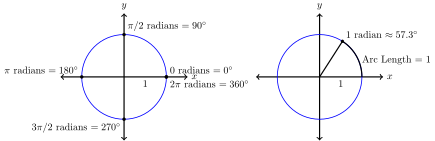
\includegraphics[width=0.9\columnwidth]{figures/0-5-fig2.pdf}
    \caption{Common radian measures.}
    \label{fig:0.5.radian}
\end{figure}

Because we define the radian in this way, this means that the arc length $s$ along the
circumference of a circle with radius $r$ over angle $\theta$ can be calculated as $s = r
\theta$ as long as the angle $\theta$ is measured in radians.

\begin{figure}
    \begin{center}
%     \begin{tikzpicture}[scale=1]
%         \draw[thick, color=blue] (0,0) circle(1.5cm);
%         \draw[color=black, very thick] (0,0) -- (0.61,1.37) arc(66:-23:1.5cm) -- (0,0);
%         \draw (0,0.1) node[anchor=west]{$\theta$};
%         \draw (1.4,0.2) node[anchor=south west]{$s$};
%         \draw (0.8,-0.3) node[anchor=north]{$r$};
%     \end{tikzpicture}
        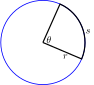
\includegraphics[width=0.3\columnwidth]{figures/0-5-fig3.pdf}
    \end{center}
    \caption{Arc length, angle, and radius on a circle.}
    \label{fig:0.5.arc}
\end{figure}


\subsection*{Sine and Cosine on the Unit Circle}

Let's draw a unit circle with its center at the origin and think about a point moving along the circumference of this circle.  We start with the point on the $x$ axis with coordinates (1,0), as shown in the figure below, and define this location to be an angle of $\theta = 0$ radians.  Then, we let this point move up, so that our point is at an angle $\theta$ above the $x$ axis.  The sine and cosine functions are defined so that they give us the coordinates of our point:   
\[ x = \cos \theta \quad \text{and} \quad y = \sin \theta \]


\begin{figure}
    \begin{center}
%     \begin{tikzpicture}[scale=1.5]
%         \draw[<->, very thick] (-1.5,0) -- (1.5,0) node[anchor=west]{$x$}; 
%         \draw[<->, very thick] (0,-1.5) -- (0,1.5) node[anchor=south]{$y$}; 
%         \draw[thick, color=blue] (0,0) circle(1cm);
%         \draw[color=black, very thick] (0,0) -- (0.54,0.84);
%         \draw[color=black,fill=black] (0.54,0.84) circle(0.04cm)
%         node[anchor=south west]{$(x,y)=(\cos\theta,\,\sin\theta)$};
%         \draw[->, thick] (0,0) -- (0.54,0);
%         \draw[->, thick] (0.54,0) -- (0.54,0.84);
%         \draw (0.26,0) node[anchor=north]{$x$};
%         \draw (0.54,0.42) node[anchor=west]{$y$};
%         \draw[color=black, fill=black] (1,0) circle(0.035cm) node[anchor=south
%         west]{$(1,0)$};
%     \end{tikzpicture}
        \includegraphics[width=0.4\columnwidth]{figures/0-5-fig4.pdf}
    \end{center}
    \caption{Sine and cosine on a unit circle.}
    \label{fig:0.5.unit}
\end{figure}

% \resizebox{4in}{!}{
% \begin{picture}(200,100)(0,0)
% \thicklines
% \put(50,50){\circle{40}}
% \put(70,50){\circle*{3}}
% \put(20,50){\line(1,0){60}}
% \put(50,20){\line(0,1){60}}
% \put(73,52){\tiny(1,0)}
% \put(130,50){\circle{40}}
% \put(143,65){\circle*{3}}
% \put(100,50){\line(1,0){60}}
% \put(130,20){\line(0,1){60}}
% \put(130,50){\line(5,6){13}}
% \put(144,67){\tiny$(x,y)=(\cos \theta, \sin \theta)$}
% \put(134,51){\tiny$\theta$}
% \put(143,50){\vector(0,1){14} }
% \put(144,53){\tiny$y$}
% \put(130,47){\vector(1,0){12} }
% \put(134,42){\tiny$x$}
% \end{picture}}

This means that an angle of $\theta = 2 \pi$ carries us around one full circle and brings
us back to our starting point on the $x$ axis again, with coordinates (1,0).  That means
that $\sin 2 \pi = \sin 0 = 0$.  Similarly $\theta = 4 \pi$ carries us around two full
circles, and $\theta = 6 \pi$ carries us around three full circles. 

Next we can use the Pythagorean Theorem, and remember that our hypotenuse is equal to one to see that
\[ \sin^2 \theta + \cos^2 \theta = 1 \]
This is a very useful relationship!

\begin{activity}\label{A:0.5.1}
    Figure \ref{fig:0.5.A1} gives us the voltage produced by an electrical circuit as a function of time.
    \begin{figure}[ht!]
    \begin{center}
%         \begin{tikzpicture}
%             \begin{axis}[axis lines=center, xmin=0, xmax=0.05, ymin=-15, ymax=55, grid,
%                     domain=0:0.05, xlabel={time (sec)}, ylabel={volts},
%                     xtick={0.005,0.01,0.015,0.02,0.025,0.03,0.035,0.04,0.045,0.05},
%                     xticklabels={0.005,0.01,0.015,0.02,0.025,0.03,0.035,0.04,0.045,0.05},
%                 ytick={-10,10,20,30,40,50}, xscale=2]
%                 \addplot[smooth, very thick, blue, samples=100]
%                 {30*sin(deg(2*pi/0.017*(x-0.008)))+20};
%             \end{axis}
%         \end{tikzpicture}
        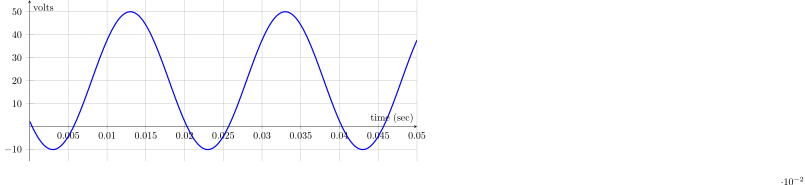
\includegraphics[trim=0cm 0cm 12cm 0cm, clip, width=0.9\columnwidth]{figures/0-5-fig9.pdf}
    \end{center}
    \caption{Voltage as a function of time.}
    \label{fig:0.5.A1}
\end{figure}
% \resizebox{5in}{!}{\includegraphics{0-5-TrigonometricFunctions5.jpg}}


\ba
\item What is the amplitude of the oscillations?  % 30 volts
\item What is the period of the oscillations? % about 0.017 seconds
\item What is the average value of the voltage?  % 20 volts
\item What is the shift along the $t$ axis, $t_0$?  % about 0.008 seconds
\item What is a formula for this function?  %  V(t) = 30 \sin( 2\pi / 0.017 ( t - 0.008) ) + 20
\ea

\end{activity}
\begin{smallhint}
    \ba
        \item measure the amplitude at half the maximum minus the minimum.
        \item measure the period from peak to peak or from trough to trough.
        \item the average value comes from the $y$ values.
        \item find the middle of the voltage values.
        \item be sure to get the shift correct.  
        \item There are infinitely many answers to this
            problem!
    \ea
\end{smallhint}
\begin{bighint}
    \ba
        \item measure the amplitude at half the maximum minus the minimum.
        \item measure the period from peak to peak or from trough to trough.
        \item the average value comes from the $y$ values.
        \item find the middle of the voltage values.
        \item be sure to get the shift correct.  
        \item There are infinitely many answers to this
            problem!
    \ea
\end{bighint}
\begin{activitySolution}
   \ba
    \item The amplitude is $A = \frac{1}{2}(50-(-10)) = 30$.
    \item The period is the distance from peak to peak.  In this case there is a peak at
        approximately $t=0.0125$ seconds and $t = 0.0325$ seconds.  Hence, the period is
        $0.02$ seconds.
    \item The average value of the voltage is 20.
    \item The simplest shift is probably to the first peak at $t = 0.0125$ seconds.
    \item $V(t) = 30 \cos\left( \frac{2\pi}{0.02} \left( t - 0.0125 \right) \right) + 20$.
   \ea
\end{activitySolution}

\aftera


\subsection*{Sine and Cosine as Functions} 

To get beyond trigonometry, rather than using the angle $\theta$ as the input to our sine
and cosine functions, instead we will put our function input on the $x$ axis.  Then we can
plot the output of on the $y$ axis.  This produces the following graph:
\begin{center}
%     \begin{tikzpicture}
%         \begin{axis}[axis lines=center, xlabel={$x$}, xmin=-7, xmax=7,
%                 ymin=-1.5, ymax=1.5, ytick={-1,1}, xtick={-6.28, -4.71, -3.14, -1.57,
%                 1.57, 3.14, 4.71, 6.28},
%             xticklabels={$-2\pi$,$-\frac{3}{2}\pi$,$-\pi$,$-\frac{1}{2}\pi$,$\frac{1}{2}\pi$,$\pi$,$\frac{3}{2}\pi$,$2\pi$},
%         grid, xscale=2]
%             \addplot[smooth, very thick, color=blue, domain=-6.5:6.5, samples=100] {sin(deg(x))};
%             \draw (axis cs:0,1) node[anchor=south west]{$y = \sin(x)$};
%         \end{axis}
%     \end{tikzpicture}
    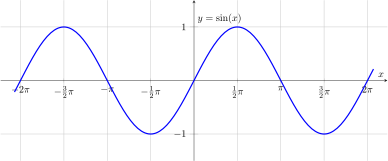
\includegraphics[width=0.85\columnwidth]{figures/0-5-fig5.pdf}
\end{center}

% \resizebox{4in}{!}{\includegraphics{0-5-TrigonometricFunctions2.jpg}}

\noindent
Here we can see that the range (output) of the sine function is the interval from $-1$ to
$+1$.  ($\sin x$ can never equal 2!)  The domain (input) of the sine function is extends
from $-\infty$ to $+\infty$, but the cycle repeats every $2 \pi$ along the $x$ axis.  (Do
you understand how the definition of sine on the unit circle makes both of these facts
true?)

The following terms will be very important when we describe functions like this:

\begin{itemize}
\item The \emph{period} of a function is how far along the $x$ axis it takes to complete one full cycle.
\item The \emph{amplitude} of a function is how far it goes on the $y$ axis above and below its average value.
\end{itemize}
The function $f(x) = \sin x$ has a period of $2 \pi$ and an amplitude of $1$.  If we plot
both the sine and the cosine functions together we see the following graph:
\begin{center}
%     \begin{tikzpicture}
%         \begin{axis}[axis lines=center, xlabel={$x$}, ylabel={$y$}, xmin=0, xmax=7,
%                 ymin=-1.25, ymax=1.25, ytick={-1,-0.5,0.5,1}, xtick={0.785,
%                 1.57, 2.356, 3.14, 3.927, 4.71, 5.498, 6.28},
%                 xticklabels={$\frac{1}{4}\pi$,$\frac{1}{2}\pi$, $\frac{3}{4}\pi$,$\pi$,
%                 $\frac{5}{4}\pi$,$\frac{3}{2}\pi$,$\frac{7}{4}\pi$,$2\pi$},
%                 yticklabels={$-1$,$-\frac{1}{2}$,$\frac{1}{2}$,$1$},
%         grid, xscale=2]
%             \addplot[smooth, very thick, color=blue, domain=0:6.5, samples=100] {sin(deg(x))};
%             \addplot[smooth, dashed, very thick, color=red, domain=0:6.5, samples=100]
%             {cos(deg(x))};
%             \draw (axis cs:2.4,0.7) node[anchor=south west]{$y = \sin(x)$};
%             \draw (axis cs:5.5,0.7) node[anchor=south east]{$y = \cos(x)$};
%         \end{axis}
%     \end{tikzpicture}
    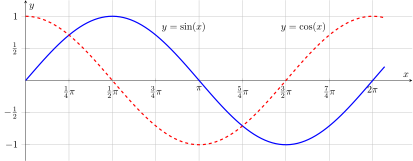
\includegraphics[width=0.85\columnwidth]{figures/0-5-fig6.pdf}
\end{center}
% \resizebox{4in}{!}{\includegraphics{0-5-TrigonometricFunctions1.jpg}}
From this we see that the function $g(x) = \cos x$ also has a period of $2 \pi$ and an
amplitude of $1$.  The difference is that $\sin 0 = 0$, so the sine function starts at its
average value, halfway between a peak and a trough.  On the other hand $\cos 0 = 1$, so
the cosine function starts at a peak.  This means that we can turn a cosine function into
a sine function and visa versa simply by shifting:
\[ \sin(x) = \cos \left( x - \frac{\pi}{2} \right) \quad \text{and} \quad \cos(x) = \sin
\left( x + \frac{\pi}{2} \right). \]


\subsection*{Sinusoidal Functions in the Real World}

To model real data with the sine function, we must be able to change the amplitude, the
period, and the average value of our wave, to get what we call a \emph{sinusoidal}
function.  Every sinusoidal function can be written either of these two forms:

% \begin{callout}
    \[ f(t) = A \sin( B ( t - t_0) ) + C \mbox{ or } f(t) = A \sin( B t + \phi) + C \]

\begin{itemize}
\item $A$ is the amplitude.  
\item $B$ is the angular frequency, which determines the period, with $B = \frac{2 \pi}{\mbox{Period}}$.  
\item $C$ is the average value.  
\item $t_0$ is the shift along the $t$ axis, a time when $f$ is at an average value and increasing
\item $\phi$ is the shift in radians, the angle at which the oscillations begin
\end{itemize}
% \end{callout}

The parameter $B$ can be a little surprising.  Because $B$ is inversely related to the
period, this means that larger values of $B$ result in a shorter period, and smaller
values of $B$ result in a longer period, as we see in the graphs below:
% \def\scl{0.89}
\begin{center}
%     \begin{tikzpicture}[scale=\scl]
%         \begin{axis}[axis lines=center, xmin=0, xmax=6.28, ymin=-1.25, ymax=1.25,
%             domain=0:6.28, xlabel={$t$}, title={$\sin(t)$}, grid, xtick={0.785,
%                 1.57, 2.356, 3.14, 3.927, 4.71, 5.498, 6.28},
%                 xticklabels={$\frac{1}{4}\pi$,$\frac{1}{2}\pi$, $\frac{3}{4}\pi$,$\pi$,
%                 $\frac{5}{4}\pi$,$\frac{3}{2}\pi$,$\frac{7}{4}\pi$,$2\pi$}]
%             \addplot[smooth, color=blue, very thick, samples=100] {sin(1*deg(x))};
%         \end{axis}
%     \end{tikzpicture}
%     \begin{tikzpicture}[scale=\scl]
%         \begin{axis}[axis lines=center, xmin=0, xmax=6.28, ymin=-1.25, ymax=1.25,
%             domain=0:6.28, xlabel={$t$}, title={$\sin(2t)$}, grid, xtick={0.785,
%                 1.57, 2.356, 3.14, 3.927, 4.71, 5.498, 6.28},
%                 xticklabels={$\frac{1}{4}\pi$,$\frac{1}{2}\pi$, $\frac{3}{4}\pi$,$\pi$,
%                 $\frac{5}{4}\pi$,$\frac{3}{2}\pi$,$\frac{7}{4}\pi$,$2\pi$}]
%             \addplot[smooth, color=blue, very thick, samples=100] {sin(2*deg(x))};
%         \end{axis}
%     \end{tikzpicture}
%     \begin{tikzpicture}[scale=\scl]
%         \begin{axis}[axis lines=center, xmin=0, xmax=6.28, ymin=-1.25, ymax=1.25,
%             domain=0:6.28, xlabel={$t$}, title={$\sin(3t)$}, grid, xtick={0.785,
%                 1.57, 2.356, 3.14, 3.927, 4.71, 5.498, 6.28},
%                 xticklabels={$\frac{1}{4}\pi$,$\frac{1}{2}\pi$, $\frac{3}{4}\pi$,$\pi$,
%                 $\frac{5}{4}\pi$,$\frac{3}{2}\pi$,$\frac{7}{4}\pi$,$2\pi$}]
%             \addplot[smooth, color=blue, very thick, samples=100] {sin(3*deg(x))};
%         \end{axis}
%     \end{tikzpicture}
%     \begin{tikzpicture}[scale=\scl]
%         \begin{axis}[axis lines=center, xmin=0, xmax=6.28, ymin=-1.25, ymax=1.25,
%             domain=0:6.28, xlabel={$t$}, title={$\sin(4t)$}, grid, xtick={0.785,
%                 1.57, 2.356, 3.14, 3.927, 4.71, 5.498, 6.28},
%                 xticklabels={$\frac{1}{4}\pi$,$\frac{1}{2}\pi$, $\frac{3}{4}\pi$,$\pi$,
%                 $\frac{5}{4}\pi$,$\frac{3}{2}\pi$,$\frac{7}{4}\pi$,$2\pi$}]
%             \addplot[smooth, color=blue, very thick, samples=100] {sin(4*deg(x))};
%         \end{axis}
%     \end{tikzpicture}
    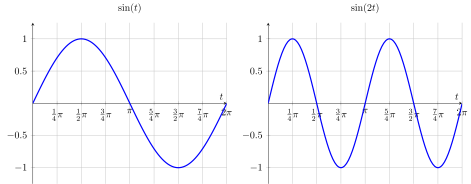
\includegraphics[width=0.99\columnwidth]{figures/0-5-fig7.pdf}
    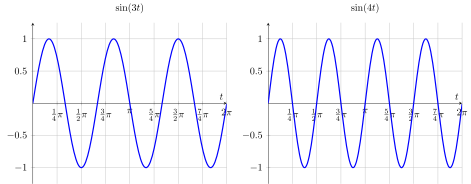
\includegraphics[width=0.99\columnwidth]{figures/0-5-fig7b.pdf}
\end{center}


% \resizebox{4in}{!}{\includegraphics{0-5-TrigonometricFunctions6.jpg}}
% 
% \resizebox{4in}{!}{\includegraphics{0-5-TrigonometricFunctions7.jpg}}
% 
% \resizebox{4in}{!}{\includegraphics{0-5-TrigonometricFunctions8.jpg}}
% 
% 
\bex
Suppose we measure the temperature every hour throughout a day and find that $T$ varies in
a smooth sinusoidal pattern.  We find that the average temperature is $60^\circ$, the
amplitude is $20^\circ$, and the period is 24 hours.  The minimum temperature is at 4am,
the maximum temperature is at 4pm, and so it is at the average temperature and increasing
at 10am.  How would we model the temperature as a sinusoidal function?
\eex
Given the information above we could model these temperatures with the following formula:
\[ T(t) = 20 \sin \left( \frac{2 \pi}{24} (t - 10) \right) + 60. \]
A graph of the function looks like this:
\begin{center}
%     \begin{tikzpicture}
%         \begin{axis}[xmin=0, xmax=50, ymin=0, ymax=100, grid,
%             domain=0:50, xlabel={time (hours)}, ylabel={Temperature ($^\circ$F)},
%         xtick={5,10,15,20,25,30,35,40,45,50}]
%             \addplot[smooth, very thick, blue, samples=100] {20*sin(deg(2*pi/24 *
%             (x-10)))+60};
%         \end{axis}
%     \end{tikzpicture}
    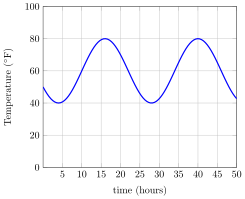
\includegraphics[width=0.5\columnwidth]{figures/0-5-fig8.pdf}
\end{center}
% \resizebox{5in}{!}{\includegraphics{0-5-TrigonometricFunctions3.jpg}}
% 
Notice that the maximum temperature is $80^\circ$ and the minimum temperature is
$40^\circ$.  We could tell this directly from the formula, because output of the sine
function varies between $-1$ and $+1$, and this is multiplied by 20.  As a result, the
most we ever add to 60 is 20 to get a maximum temperature of 80, and the most we ever
subtract from 60 is 20, to get a minimum temperature of 40.

\afterex

\begin{activity}\label{A:0.5.2}
Suppose the following sinusoidal function models the water level on a pier in the ocean as
it changes due to the tides during a certain day.
\[ w(t) = 4.3 \sin \left( 0.51 t + 0.82 \right) + 10.6 \]
\ba
\item Using the formula above, make a table showing the water level every two hours for a 24 hour period starting at midnight.
    \begin{center}
        \begin{tabular}[h!]{|c||c|c|c|c|c|c|c|c|c|c|c|c|c|}
            \hline
            time (hours) & 0 & 2 & 4 & 6 & 8 & 10 & 12 & 14 & 16 & 18 & 20 & 22 & 24 \\
            \hline
            water level (ft) & & & & & & & & & & & & & \\ \hline
        \end{tabular}
    \end{center}
\item Sketch a graph of this function using the data from your table in part (a).
    \begin{center}
%         \begin{tikzpicture}
%             \begin{axis}[ymin=0, ymax=20, xmin=0, xmax=24, domain=0:24,
%                 grid, xtick={2,4,6,8,10,12,14,16,18,20,22,24},
%             ytick={0,2,4,6,8,10,12,14,16,18,20}, xlabel={time (hours)}, ylabel={water level
%             (ft)}, xscale=1.25]
%                 \addplot[smooth] {0*x};
%             \end{axis}
%         \end{tikzpicture}
        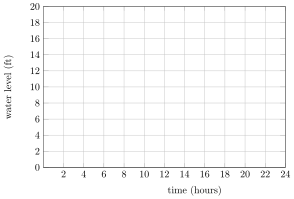
\includegraphics[width=0.6\columnwidth]{figures/0-5-fig10.pdf}
    \end{center}
\item What is the period of oscillation of this function? % Period $ = 2 \pi / B \approx  12.3$ hours.
\item What time is high tide?  % The sine function reaches a peak when its input is $\pi/2$.  So $0.51 t + 0.82 = \pi/2$ and $t = 1.47$ hours, or about 1:30 am.

\ea
\end{activity}\aftera







% \subsection*{Units}
% 
% Whenever we use mathematics in the real world, most numbers have units, like meters,
% minutes, dollars, pounds, or degrees.  Units are a very useful tool that helps us
% understand the meaning of the numbers that we are using.  For example, suppose we use the
% following sinusoidal function to model the water level on a pier in the ocean as it
% changes due to the tides during a certain day.
% \[ w(t) = 4.3 \sin \left( 0.51 t + 0.82 \right) + 10.6 \]
% This function isn't very useful to us unless we know what units the input $t$ must have
% (Minutes?  Seconds?  Hours?  Days?) and what units the output $w$ will have (Centimeters?
% Feet?  Meters?  Yards?).  In this case $t$ is in hours since midnight, and $w$ is in feet.
% Now, we can evaluate the function at noon to find that the water level is $w(12) = 13.3$
% feet.
% 
% % \begin{callout}
%     Here's how units work in equations:  
%     \begin{itemize}
%         \item If two numbers are equal, or if we add or subtract
%             two numbers, they must have the same units:  3 seconds plus 5 feet doesn't make any sense.
%         \item If we multiply or divide two numbers, both units go into the result:  6 meters divided by
%             2 seconds equals a speed of 3 meters per second. 
%     \end{itemize}
% % \end{callout}
% 
% The parameters in our water level function ($A = 4.3$, $B = 0.51$, $\phi = 0.82$, $C =
% 10.6$) all have units, which help us interpret their meaning.   The sine, cosine, and
% tangent functions all take angles in radians as their input, and return numbers with no
% units as output.  $C = 10.6$ must be in feet, because we add it to something else, and
% then it equals the output, which is in feet.  Similarly $A = 4.3$ must also be in feet,
% because the sine function does not have any units on its output.  $\phi = 0.82$ must be in
% radians, because we add it to something else and use it as input to the sine function.
% Similarly $0.51 t$ must be in radians.  However, we know that $t$ is in hours, so $B =
% 0.51$ must have units of radians per second.  
% 
% 
% 


\input{activities/0.5.Act3}






\subsection*{The Tangent Function}

The tangent function has a completely different shape than the sine and cosine functions because it is defined to be
\[ \tan \theta = \frac{\sin \theta}{\cos \theta} \]
as long as $\cos \theta \neq 0$, so that we don't have a divide-by-zero problem.  This
means that the tangent function is undefined at $\pm \pi/2, \pm 3 \pi/2, \cdots$, and the
function has vertical asymptotes at these points.
\begin{center}
%     \begin{tikzpicture}
%         \begin{axis}[axis lines=center, xlabel={$x$}, xmin=-7, xmax=7,
%                 ymin=-1.5, ymax=1.5, ytick={-1,1}, xtick={-6.28, -4.71, -3.14, -1.57,
%                 1.57, 3.14, 4.71, 6.28},
%             xticklabels={$-2\pi$,$-\frac{3}{2}\pi$,$-\pi$,$-\frac{1}{2}\pi$,$\frac{1}{2}\pi$,$\pi$,$\frac{3}{2}\pi$,$2\pi$},
%         grid, xscale=2, restrict y to domain=-3:3]
%             \addplot[smooth, very thick, color=blue, domain=-6.5:6.5, samples=100] {tan(deg(x))};
%             \draw (axis cs:1.7,1) node[anchor=south west]{$y = \tan(x)$};
%             \draw[thick, dashed] (axis cs:-4.71,-1.5) -- (axis cs:-4.71,1.5);
%             \draw[thick, dashed] (axis cs:4.71,-1.5) -- (axis cs:4.71,1.5);
%             \draw[thick, dashed] (axis cs:-1.57,-1.5) -- (axis cs:-1.57,1.5);
%             \draw[thick, dashed] (axis cs:1.57,-1.5) -- (axis cs:1.57,1.5);
%         \end{axis}
%     \end{tikzpicture}
    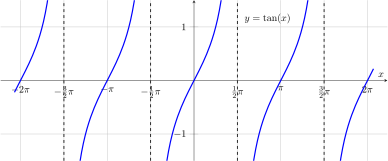
\includegraphics[width=0.8\columnwidth]{figures/0-5-fig11.pdf}
\end{center}
% \resizebox{3in}{!}{\includegraphics{0-5-TrigonometricFunctions9.jpg}}
Because the tangent function blows up to infinity, we don't often fit tangent functions to real world data.

\subsection*{Inverse Sine, Cosine, and Tangent Functions}

Suppose we want to find the value of $x$ so that $\sin x = 0.75$.  To find this, we use an
inverse sine function, written as either $\arcsin$ or $\sin^{-1}$.  In this case
$\sin^{-1} 0.75 \approx 0.848$, because $\sin 0.848 \approx 0.75$.  The range of the sine
function only goes from $-1$ to $+1$, so that means the domain of $\arcsin$ only goes from
$-1$ to $+1$.  It is impossible to find a solution to $\sin x = 3$, because the sine
function doesn't go that high!

It is important to remember that the sine function repeats itself in the same pattern
again and again, every $2\pi$, so $x = 0.848$ is not the only solution to $\sin x = 0.75$.
Another solution is $x = 0.848 + 2 \pi \approx 7.13$.  Another solution is $x = 0.848 + 4
\pi \approx 13.4.$.  And of course we could subtract multiples of $2 \pi$ as well to get
$x = 0.848 - 2 \pi \approx -5.44$.  As a result, we have the $\arcsin$ function output the
value between $-\pi/2$ and $+\pi/2$.  This means that the arcsine function has a very
limited domain and range, only existing for $ -1 \leq x \leq 1$ and $-\pi/2 \leq y \leq
\pi/2$.
% \begin{center}
%     \begin{tikzpicture}
%         \draw[thick, <->] (-2,0) -- (2,0) node[anchor=west]{$x$};
%         \draw[thick, <->] (0,-2.25) -- (0,2.25) node[anchor=south]{$y=\sin^{-1}(x)$};
%         \draw[color=blue, very thick, domain=-1.57:1.57] plot ({sin(deg(\x))},{\x});
%         \draw (1,0) node[anchor=north]{$1$};
%         \draw (-1,0) node[anchor=south]{$-1$};
%         \draw (0,1.57) node[anchor=east]{$\pi/2$};
%         \draw (0,-1.57) node[anchor=west]{$-\pi/2$};
%         \draw[thick, dashed] (1,0) -- (1,1.57) -- (0,1.57);
%         \draw[thick, dashed] (-1,0) -- (-1,-1.57) -- (0,-1.57);
%         \draw (0,-2.25) node[anchor=north]{Domain: $-1\le x \le 1$, Range: $-\pi/2 \le y
%         \le \pi/2$};
%     \end{tikzpicture}
% \end{center}

% \resizebox{2in}{!}{\includegraphics{0-5-TrigonometricFunctions10.jpg}}
Warning:  Even though we write the inverse sine function as $\sin^{-1} x$, it is a completely different thing than $1 / \sin x$.
\[ \sin^{-1}x \neq \frac{1}{\sin x} \]

% \subsection*{Inverse Cosine Function}

We can define a similar inverse function for the cosine, which we call $\arccos$ or
$\cos^{-1}$.  The domain of this function is $-1 \leq x \leq 1$, and we choose the range
to be $0 \leq y \leq \pi$.
% \begin{center}
%     \begin{tikzpicture}
%         \draw[thick, <->] (-2,0) -- (2,0) node[anchor=west]{$x$};
%         \draw[thick, <->] (0,-1) -- (0,4) node[anchor=south]{$y=\cos^{-1}(x)$};
%         \draw[color=blue, very thick, domain=0:3.14] plot ({cos(deg(\x))},{\x});
%         \draw (1,0) node[anchor=north]{$1$};
%         \draw (-1,0) node[anchor=north]{$-1$};
%         \draw (0,3.14) node[anchor=west]{$\pi$};
%         \draw[thick, dashed] (-1,0) -- (-1,3.14) -- (0,3.14);
%         \draw (0,-1) node[anchor=north]{Domain: $-1\le x \le 1$, Range: $0 \le y
%         \le \pi$};
%     \end{tikzpicture}
% \end{center}

% \resizebox{2in}{!}{\includegraphics{0-5-TrigonometricFunctions11.jpg}}

% \subsection*{Inverse Tangent Function}

Recall that the tangent function has a range going all the way from negative infinity to
positive infinity, as $x$ goes from $-\pi/2$ to $+\pi/2$.  As a result, the inverse
tangent function has a domain of $-\infty < x < \infty$, and a range of $-\pi/2 \leq y
\leq \pi/2$.  The three primary inverse trigonometric functions are shown in Figure
\ref{F:0.5.inverse_trig}.

% \begin{center}
%     \begin{tikzpicture}
%         \draw[thick, <->] (-3,0) -- (3,0) node[anchor=west]{$x$};
%         \draw[thick, <->] (0,-2.25) -- (0,2.25) node[anchor=south]{$y=\tan^{-1}(x)$};
%         \draw[color=blue, very thick, domain=-1.25:1.25] plot ({tan(deg(\x))},{\x});
%         \draw (0,1.57) node[anchor=south east]{$\pi/2$};
%         \draw (0,-1.57) node[anchor=north west]{$-\pi/2$};
%         \draw[thick, dashed] (-3,1.57) -- (3,1.57);
%         \draw[thick, dashed] (-3,-1.57) -- (3,-1.57);
%         \draw (0,-2.25) node[anchor=north]{Domain: $\mathbb{R}$, Range: $-\pi/2 < y
%         < \pi/2$};
%     \end{tikzpicture}
% \end{center}
% \resizebox{2in}{!}{\includegraphics{0-5-TrigonometricFunctions12.jpg}}
% 
% 
\begin{figure}[ht!]
    \begin{center}
        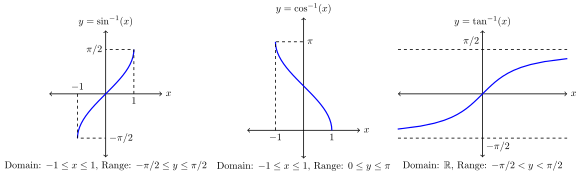
\includegraphics[width=1\columnwidth]{figures/0-5-fig12.pdf}
    \end{center}
    \caption{The inverse trigonometric functions}
    \label{F:0.5.inverse_trig}
\end{figure}


\clearpage


\begin{summary}
\item Trigonometric functions are utilized to model periodic behavior such as tides,
    sound waves, or voltage through an electrical circuit.
\item Converting between radian measure and degree measure can be achieved by remembering
    that
    \[ 2\pi \text{ radians} = 360^\circ \]
\item for $f(t) = A \sin( B ( t - t_0) ) + C$ or $f(t) = A \sin( B t + \phi) + C$
\begin{itemize}
\item $A$ is the amplitude.  
\item $B$ is the angular frequency, which determines the period, with $B = \frac{2 \pi}{\mbox{Period}}$.  
\item $C$ is the average value.  
\item $t_0$ is the shift along the $t$ axis, a time when $f$ is at an average value and increasing
\item $\phi$ is the shift in radians, the angle at which the oscillations begin
\end{itemize}
\end{summary}


% exercises go here
\begin{exercises} 

\item What is the formula for a sinusoidal function that has a minimum at coordinates
    $(3,6)$ followed by a maximum at $(5,9)$?  %  1.5 \sin(\frac{ \pi}{2} (x-3)) + 7.5 
\begin{exerciseSolution}
\end{exerciseSolution}


\item If we take a sinusoidal function $f(t)= A \sin ( B (t - t_0)) + C$ and replace one of
    the parameters with a another function, say a linear function, we can create more
    complicated shapes.  Find formulas for the function plotted in the following graphs.

    \def\scl{0.9}
    \begin{center}
        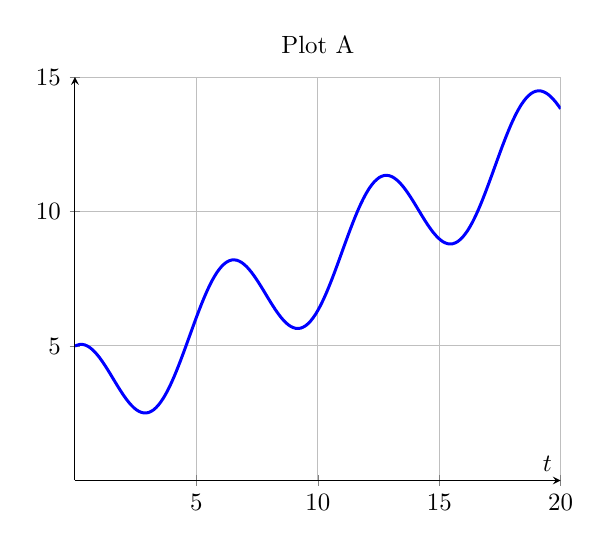
\begin{tikzpicture}[scale=\scl]
            \begin{axis}[axis lines=center, xmin=0, xmax=20, ymin=0, ymax=15, domain=0:20,
                xlabel={$t$}, title={Plot A}, grid]
                \addplot[smooth, blue, very thick, samples=100] {2*cos(deg(x)) + 3 + 0.5*x};
            \end{axis}
        \end{tikzpicture}
        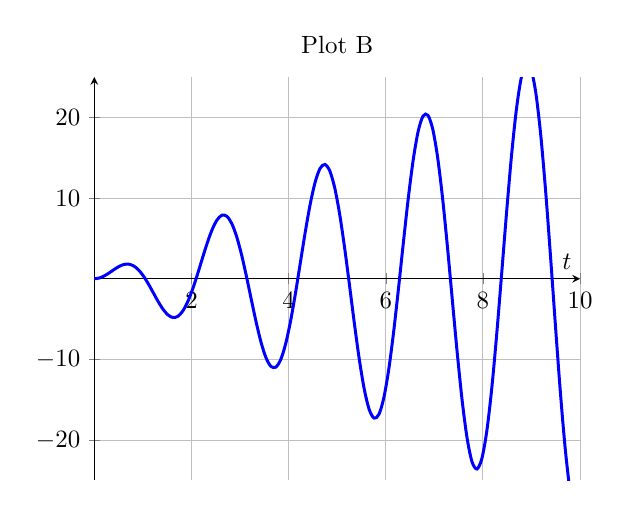
\begin{tikzpicture}[scale=\scl]
            \begin{axis}[axis lines=center, xmin=0, xmax=10, ymin=-25, ymax=25, domain=0:10,
                xlabel={$t$}, title={Plot B}, grid]
                \addplot[smooth, blue, very thick, samples=100] {3*x*sin(deg(3*x))};
            \end{axis}
        \end{tikzpicture}
        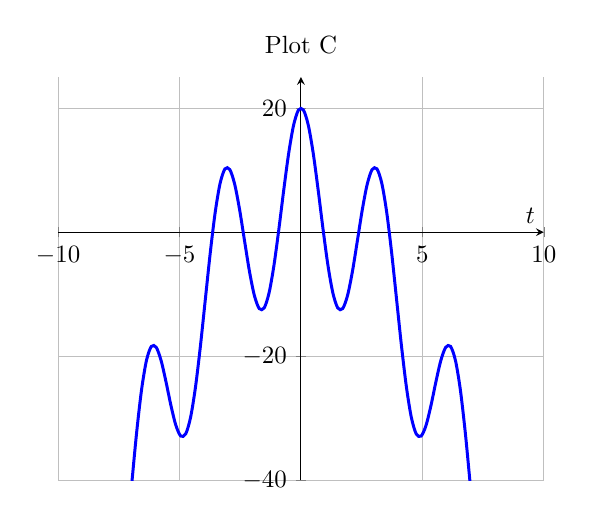
\begin{tikzpicture}[scale=\scl]
            \begin{axis}[axis lines=center, xmin=-10, xmax=10, ymin=-40, ymax=25, domain=-10:10,
                xlabel={$t$}, title={Plot C}, grid]
                \addplot[smooth, blue, very thick, samples=100] {15*cos(deg(2*x))+5-x^2};
            \end{axis}
        \end{tikzpicture}
        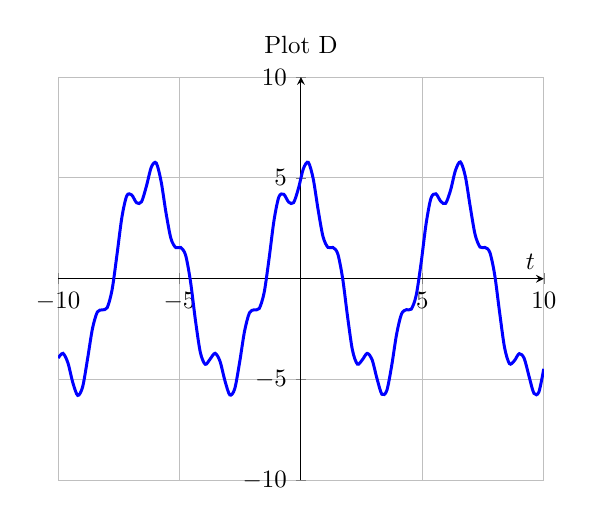
\begin{tikzpicture}[scale=\scl]
            \begin{axis}[axis lines=center, xmin=-10, xmax=10, ymin=-10, ymax=10, domain=-10:10,
                xlabel={$t$}, title={Plot D}, grid]
                \addplot[smooth, blue, very thick, samples=100]
                {5*cos(deg(x))+1*sin(deg(5*x))};
            \end{axis}
        \end{tikzpicture}
    \end{center}
\begin{exerciseSolution}
    \ba
        \item $f(t) = 2\cos(t) + 3 + 0.5*t$ over the range $[0,20]$
        \item $f(t) = 3t \sin(3t)$ over the range $[0,10]$
        \item $f(t) = 15\cos(2t) + 5-t^2$ over $[-10,10]$
        \item $f(t) = 5\cos(t) + \sin(5t)$
    \ea
\end{exerciseSolution}


\item The number of hours of daylight varies sinusoidally throughout the year.  The
    maximum occurs on the summer solstice, June 21, when we have 15 hours and 50 minutes
    of daylight.  The minimum occurs on the winter solstice, December 21, when we have
    only 8 hours and 33 minutes of daylight.  Find the formula for a function to describe
    this.  The input to your function should be $d$, the number of days since the
    beginning of the year, so that $d = 5$ on January 5.  The output of your function
    should be the amount of daylight, in minutes.  Assume that this is not a leap year.
    Hint:  Because we know the date of maximum, it is easier to write this in terms of a
    cosine function.
    % f(d) = 218.5 cos( \frac{2 \pi}{365} (d – 172) ) + 731.5

\begin{exerciseSolution}
\end{exerciseSolution}



\end{exercises}
\afterexercises





\clearpage
